\documentclass[aspectratio=169]{beamer}
\usepackage{color,amsmath}
\usepackage{subfigure}
\usepackage{booktabs}
\usepackage{framed}
\usepackage{comment}
\usepackage{url}

\definecolor{links}{HTML}{2A1B81}
\hypersetup{colorlinks,urlcolor=links}

%%%%%%%%%%%%%%%%%%%%%%%%%%
\title[]{Introduction to open-sourcing data}
\author[]{Matthew J. Salganik\\Department of Sociology\\Princeton University}
\date[]{Summer Institutes in Computational Social Science\\June 20, 2019
\vfill
\begin{flushleft}
{\scriptsize
The Summer Institutes in Computational Social Science is supported by grants from the Russell Sage Foundation and the Alfred P. Sloan Foundation.}
\end{flushleft}
\begin{flushright}

\includegraphics[width=0.1\textwidth]{figures/cc-by.png}
\end{flushright}
}
\begin{document}
%%%%%%%%%%%%%%%%%%%%%%%%%%
\frame{\titlepage}
%%%%%%%%%%%%%%%%%%%%%%%%%%
\begin{frame}

To wrap-up activity:
\begin{itemize}
\item Pay your MTurk workers
\item document and release your data to your local organizer
\end{itemize}

\end{frame}
%%%%%%%%%%%%%%%%%%%%%%%%%%
\begin{frame}

\begin{figure}
  \centering
  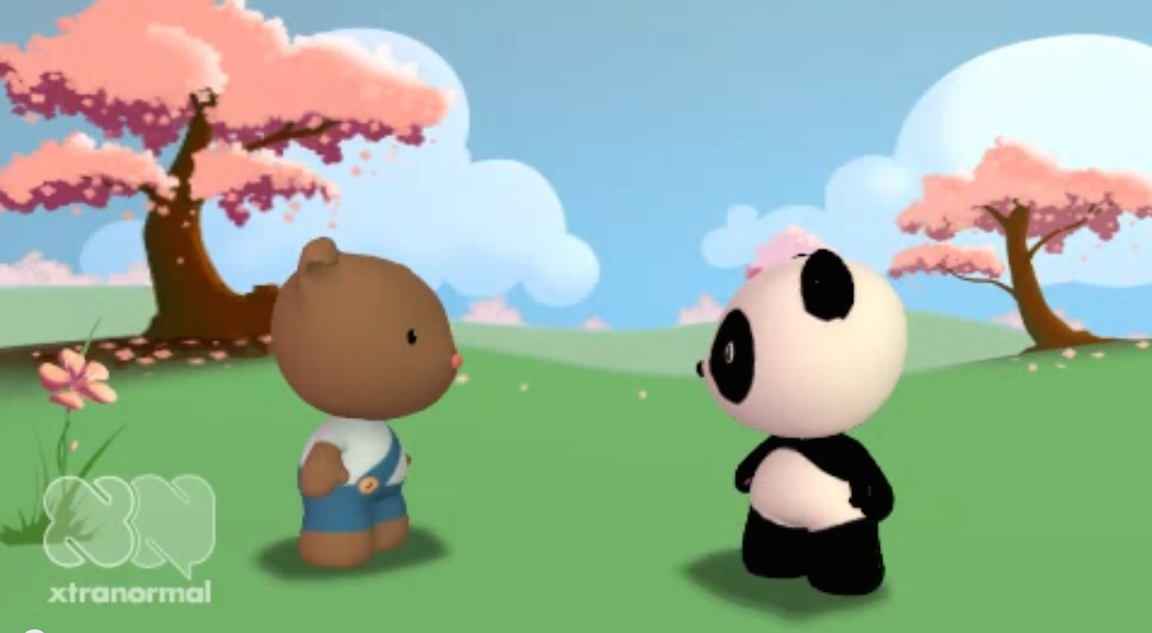
\includegraphics[width=0.9\textwidth]{figures/pandas_video}
\end{figure}

\url{https://www.youtube.com/watch?v=66oNv_DJuPc}

\end{frame}
%%%%%%%%%%%%%%%%%%%%%%%%%%%%%%%%
\begin{frame}

Brief introduction into open-sourcing your data:
\begin{itemize}
\item Store your data in a simple format
\pause
\item Provide documentation
\pause
\item Beware of privacy
\end{itemize}

\end{frame}
%%%%%%%%%%%%%%%%%%%%%%%%%%
\begin{frame}
\frametitle{Beware of privacy}
\pause

Risks come from combining data sources\\
\vfill
\begin{minipage}[c]{0.35\textwidth}
$\underbrace{\text{Baking soda}}_{\text{Safe}} + \underbrace{\text{Vinegar}}_{\text{Safe}} =$
\end{minipage}
\hspace{0.05\textwidth}
\begin{minipage}[c]{0.55\textwidth}
\onslide<2>{
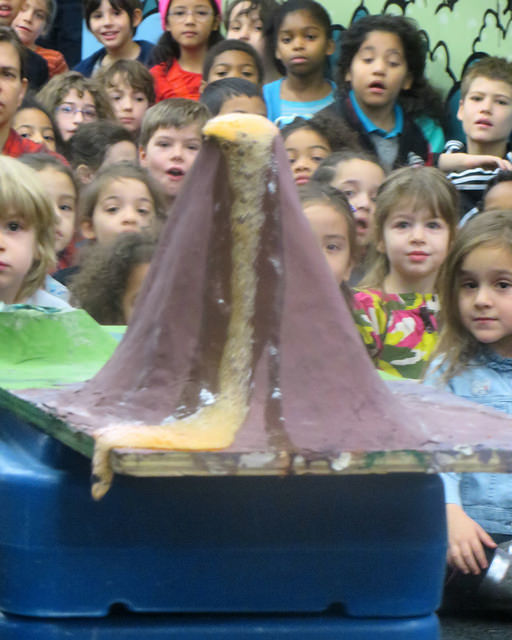
\includegraphics[width=0.8\textwidth]{figures/baking_soda_volcano}\\ {\tiny \url{https://www.flickr.com/photos/edenpictures/15962352215/}}
}
\end{minipage}

\end{frame}
%%%%%%%%%%%%%%%%%%%%%%%%%%
\begin{frame}
\frametitle{Beware of privacy}

Remove personally identifying information and/or information that could be used for linking

\begin{figure}
  \centering
  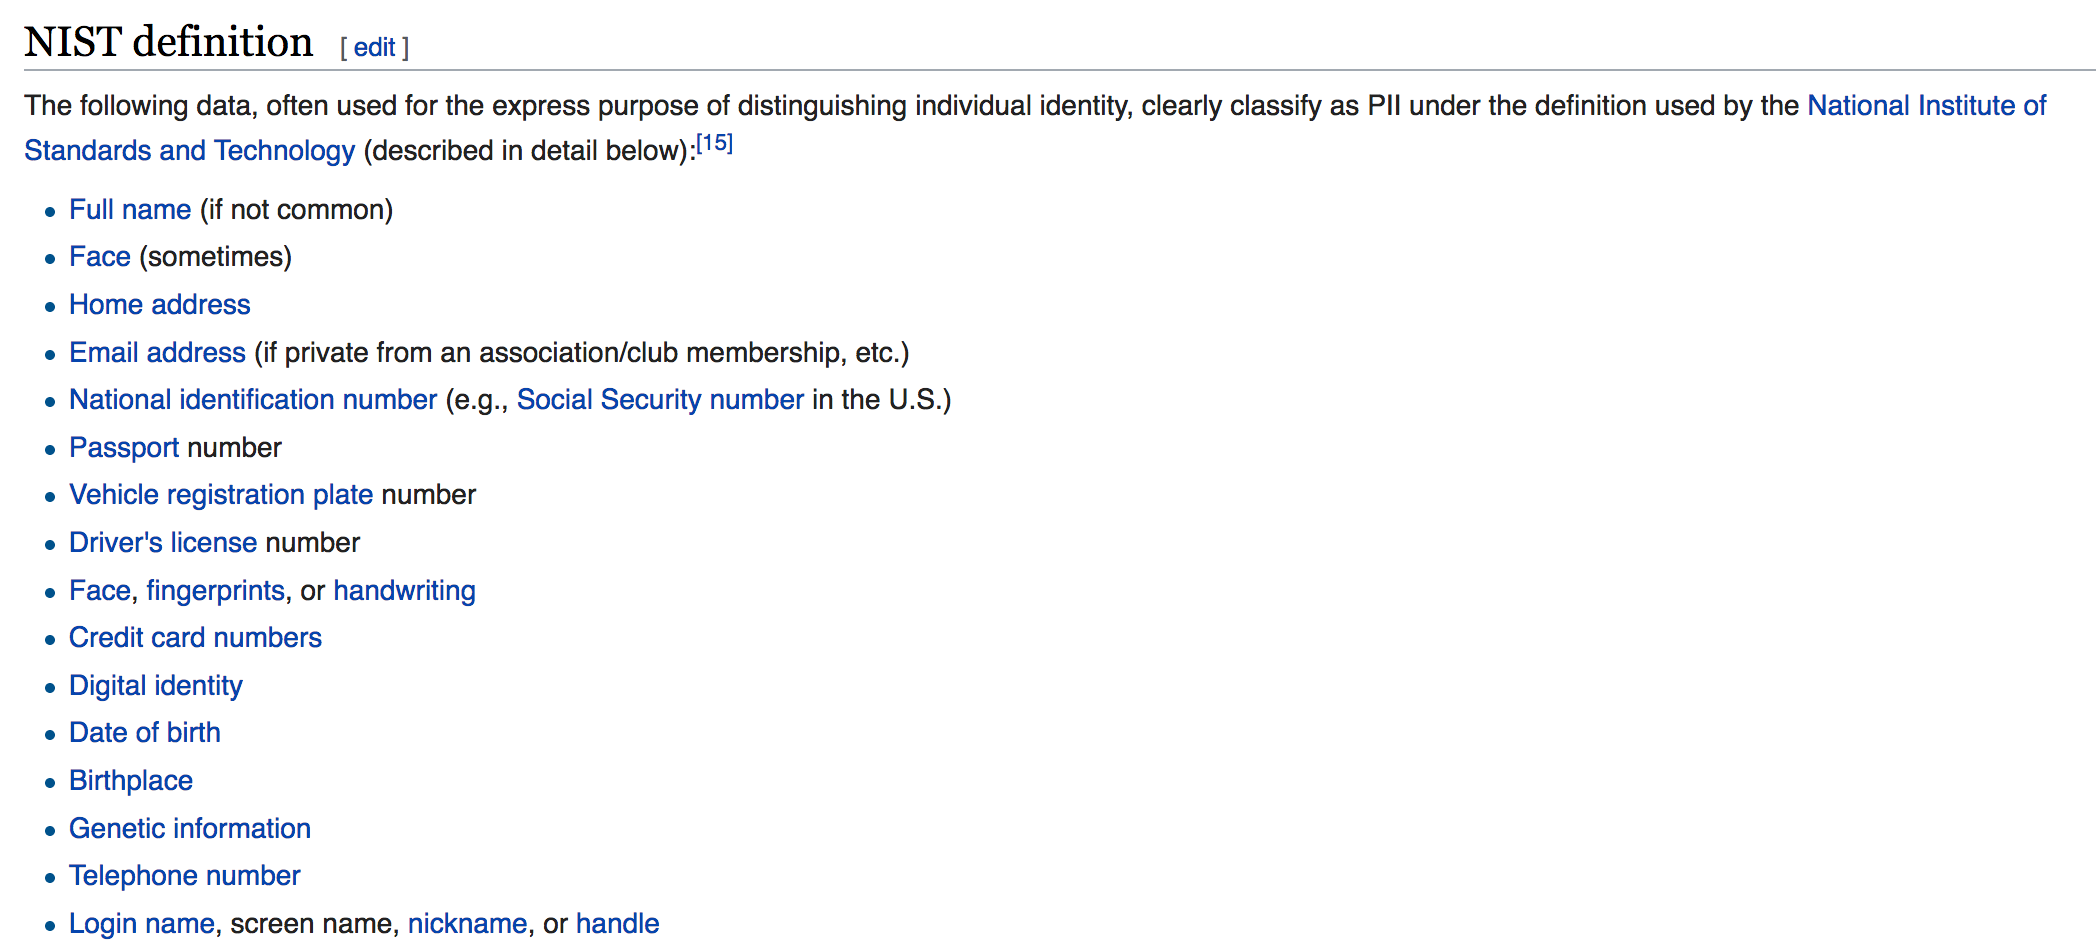
\includegraphics[width=0.9\textwidth]{figures/pii_nist}
\end{figure}

\vfill
\url{https://en.wikipedia.org/wiki/Personally_identifiable_information}

\end{frame}
%%%%%%%%%%%%%%%%%%%%%%%%
\begin{frame}

\begin{figure}
  \centering
  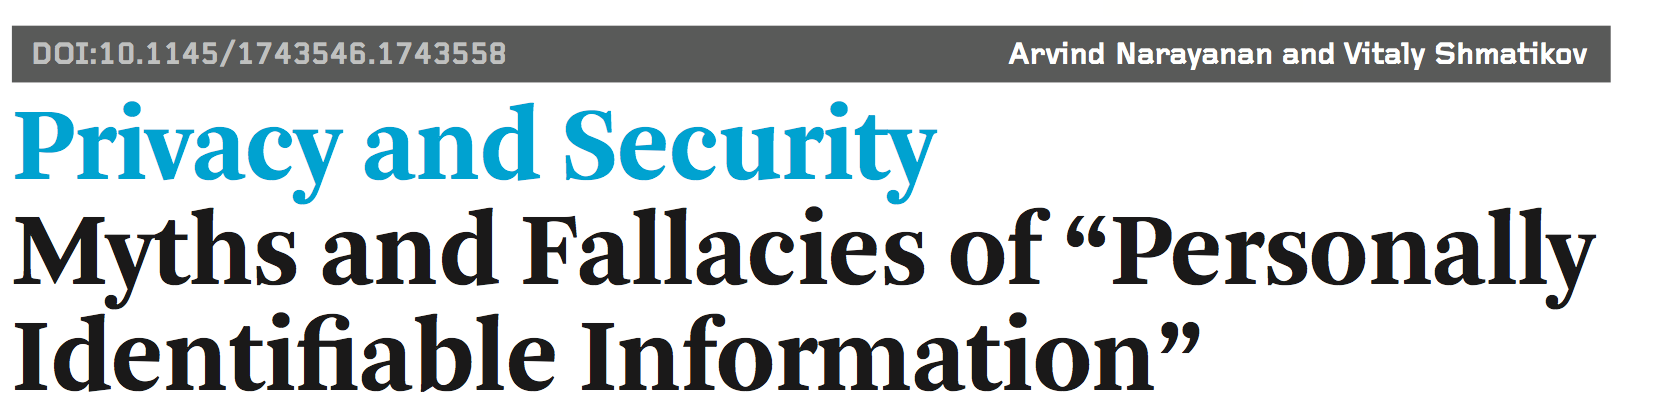
\includegraphics[width=0.9\textwidth]{figures/narayanan_myths_2010_title}
\end{figure}

\vfill
\url{http://dx.doi.org/10.1145/1743546.1743558}
\end{frame}
%%%%%%%%%%%%%%%%%%%%%
\begin{frame}

In this case, we recommend:
\begin{itemize}
\item Removing PII (name, email address, etc)
\item Removing TurkID
\item Coarsen age, geography, and race/ethnicity
\item Coarsen timestamp
\item Anything else?
\end{itemize}

For more on coarsening, see this code:\\
\url{https://github.com/compsocialscience/summer-institute/blob/master/2019/materials/day4-surveys/activity/mturk_data_cleaning.Rmd}

\end{frame}
%%%%%%%%%%%%%%%%%%%%%%%%%%
\begin{frame}

For more about de-identification, see 
\begin{itemize}
\item \textit{Bit by Bit}, Sec 6.6.2 \href{https://www.bitbybitbook.com/en/1st-ed/ethics/dilemmas/info-risk/}{\textcolor{blue}{``Understanding and managing informational risk''}}
\item Lundberg, Levy, Narayanan, Salganik (2019) ``\href{https://arxiv.org/abs/1809.00103}{Privacy, ethics, and data access: A case study of the Fragile Families Challenge'}'
\end{itemize}

\end{frame}
%%%%%%%%%%%%%%%%%%%%%%%%%%
\begin{frame}

In this case, you should share your data with your local organizer who can post it here:
\url{https://github.com/compsocialscience/summer-institute/tree/master/2019/materials/day4-surveys/datasets}

\end{frame}
%%%%%%%%%%%%%%%%%%%%%%%%%%
\begin{frame}

When you start your projects next week
\begin{itemize}
\item plan to release your data
\item plan to release your code
\end{itemize}

\end{frame}
%%%%%%%%%%%%%%%%%%%%%%%%%%
\begin{frame}

\begin{center}
\LARGE Questions
\end{center}

\end{frame}
%%%%%%%%%%%%%%%%%%%%%%%%%%


\end{document}
